% ===================================================================
%  Week 16 — Session 2: The DocScan Capstone
%  Compile: pdflatex -interaction=nonstopmode slides-b.tex  (twice)
% ===================================================================
\documentclass[10pt,aspectratio=169]{beamer}
% ===================================================================
%  Shared Beamer preamble for "Practical Image Processing"
%  English slides. Compile with pdfLaTeX.
% ===================================================================

\usetheme{metropolis}
\usepackage[T1]{fontenc}
\usepackage[utf8]{inputenc}
\usepackage{lmodern}
\usepackage{listings}
\usepackage{tcolorbox}
\usepackage{fontawesome5}
\usepackage{booktabs}
\usepackage{amsmath,amssymb}
\usepackage{tikz}
\usepackage{pgfplots}
\pgfplotsset{compat=1.17}
\usetikzlibrary{arrows.meta,positioning,shapes.geometric,fit,backgrounds,matrix}
\tcbuselibrary{skins,breakable}

% ---- Palette --------------------------------------------------------
\definecolor{coursePrimary}{HTML}{1B4965}   % deep blue
\definecolor{courseAccent}{HTML}{E76F51}    % coral
\definecolor{courseGood}{HTML}{2A9D8F}      % teal
\definecolor{courseBad}{HTML}{C0392B}       % red
\definecolor{courseInfo}{HTML}{2980B9}      % blue
\definecolor{codeBg}{HTML}{F5F6FA}
\definecolor{codeKw}{HTML}{8E44AD}
\definecolor{codeStr}{HTML}{2A9D8F}
\definecolor{codeCom}{HTML}{7F8C8D}

\setbeamercolor{frametitle}{bg=coursePrimary}
\setbeamercolor{progress bar}{fg=courseAccent}
\setbeamercolor{alerted text}{fg=courseAccent}
\metroset{block=fill,sectionpage=progressbar,numbering=fraction}

% ---- Code listings (Python is built into listings) -----------------
\lstdefinestyle{course}{
  backgroundcolor=\color{codeBg},
  basicstyle=\ttfamily\scriptsize,
  keywordstyle=\color{codeKw}\bfseries,
  stringstyle=\color{codeStr},
  commentstyle=\color{codeCom}\itshape,
  numberstyle=\tiny\color{codeCom},
  numbers=left, numbersep=6pt,
  showstringspaces=false, breaklines=true, breakatwhitespace=true,
  tabsize=4, columns=fullflexible,
  frame=single, framesep=4pt, rulecolor=\color{gray!30},
  keepspaces=true, upquote=true, language=Python,
}
\lstset{style=course}
\lstdefinelanguage{bash}{
  keywords={cd,pip,python,venv,source,import}, sensitive=true,
  morecomment=[l]{\#}, morestring=[b]', morestring=[b]",
}

% ---- Reusable callout boxes ----------------------------------------
\newtcolorbox{goodbox}[1][Good practice]{colback=courseGood!8,colframe=courseGood,
  fonttitle=\bfseries,title={\faCheck~#1},boxrule=0.6pt,left=4pt,right=4pt,top=3pt,bottom=3pt}
\newtcolorbox{badbox}[1][Pitfall]{colback=courseBad!8,colframe=courseBad,
  fonttitle=\bfseries,title={\faTimes~#1},boxrule=0.6pt,left=4pt,right=4pt,top=3pt,bottom=3pt}
\newtcolorbox{infobox}[1][Note]{colback=courseInfo!8,colframe=courseInfo,
  fonttitle=\bfseries,title={\faInfoCircle~#1},boxrule=0.6pt,left=4pt,right=4pt,top=3pt,bottom=3pt}
\newtcolorbox{mathbox}[1][Math]{colback=coursePrimary!6,colframe=coursePrimary,
  fonttitle=\bfseries,title={\faCalculator~#1},boxrule=0.6pt,left=4pt,right=4pt,top=3pt,bottom=3pt}

\newcommand{\keyidea}[1]{\begin{alertblock}{Key idea}#1\end{alertblock}}
\newcommand{\term}[1]{\textbf{\color{coursePrimary}#1}}
\newcommand{\code}[1]{\lstinline[basicstyle=\ttfamily\small]|#1|}

% ---- A helper to draw a small pixel grid, cells shaded by value ----
% \pixelgrid{ {10,20,120,200,240}, {30,60,130,180,230}, ... }
\newcommand{\pixelgrid}[1]{%
  \begin{tikzpicture}[font=\scriptsize,scale=0.6]
    \foreach \row [count=\ry] in {#1} {
      \foreach \val [count=\cx] in \row {
        \draw[gray,fill=coursePrimary!8] (\cx,-\ry) rectangle ++(1,-1);
        \node at (\cx+0.5,-\ry-0.5) {\val};
      }
    }
  \end{tikzpicture}}


\title{Transfer Learning \& the DocScan Capstone}
\subtitle{Week 16 — Session 2: Shipping the project}
\author{Practical Image Processing}
\date{Lecture 16.2 \textbullet\ 60--70 min}

\begin{document}

\maketitle

\begin{frame}{Recap of Session 1}
  \begin{columns}[T]
    \begin{column}{0.58\textwidth}
      \begin{itemize}
        \item Small data ($180$ images) $\rightarrow$ can't train a big CNN from scratch.
        \item \term{Transfer learning}: freeze a pretrained net, use it as a feature extractor.
        \item Same SVM, deep features instead of HOG: \textbf{0.48 $\rightarrow$ 0.87}.
        \item Augmentation + the backbone's own preprocessing squeeze out the rest.
      \end{itemize}
    \end{column}
    \begin{column}{0.42\textwidth}
      \begin{alertblock}{Today}
        We can read digits. Now assemble the \term{whole DocScan pipeline} and engineer it
        to survive the real world — then ship the capstone.
      \end{alertblock}
    \end{column}
  \end{columns}
\end{frame}

\begin{frame}{Roadmap}\tableofcontents\end{frame}

% ==================================================================
\section{Fine-tuning: the deeper option}
% ==================================================================

\begin{frame}{When feature extraction isn't enough}
  \begin{itemize}
    \item Feature extraction keeps the backbone \emph{fixed} — great for tiny data.
    \item With more data (thousands of images) you can \term{fine-tune}: let some top layers
          adapt to your domain.
    \item This adjusts mid/late features toward \emph{your} task, not ImageNet's 1000 classes.
  \end{itemize}
  \keyidea{Fine-tuning trades data and compute for a few extra points of accuracy — spend it only when you have the data.}
\end{frame}

\begin{frame}{The fine-tuning recipe}
  \begin{columns}[T]
    \begin{column}{0.55\textwidth}
      \begin{enumerate}
        \item Start from the pretrained weights (never random).
        \item Replace the classifier head for your classes.
        \item \term{Freeze} early layers; unfreeze the top $k$.
        \item Train with a \emph{small} learning rate ($10^{-4}$ or less).
        \item Stop early — watch the validation curve.
      \end{enumerate}
    \end{column}
    \begin{column}{0.45\textwidth}
      \begin{mathbox}[Why a small LR]
        The pretrained weights are already good. A large step
        \[ w \leftarrow w - \eta\,\nabla \]
        with big $\eta$ would erase what the giant learned.
      \end{mathbox}
    \end{column}
  \end{columns}
  \begin{badbox}
    A big learning rate on a pretrained net is \term{catastrophic forgetting} — you destroy the transfer.
  \end{badbox}
\end{frame}

\begin{frame}{Freeze depth vs.\ data size}
  \begin{center}
  \begin{tabular}{@{}lll@{}}
    \toprule
    \textbf{Data you have} & \textbf{Strategy} & \textbf{Unfreeze} \\
    \midrule
    hundreds & feature extraction & nothing (frozen) \\
    a few thousand & fine-tune top block & last 1--2 stages \\
    tens of thousands & fine-tune widely & most of the net \\
    millions & train from scratch is viable & everything \\
    \bottomrule
  \end{tabular}
  \end{center}
  \begin{goodbox}
    Our DocScan digits use \emph{feature extraction} — hundreds of samples, small domain gap.
  \end{goodbox}
\end{frame}

% ==================================================================
\section{The DocScan capstone}
% ==================================================================

\begin{frame}{DocScan: the whole course in one pipeline}
  \begin{columns}[T]
    \begin{column}{0.34\textwidth}\begin{center}
      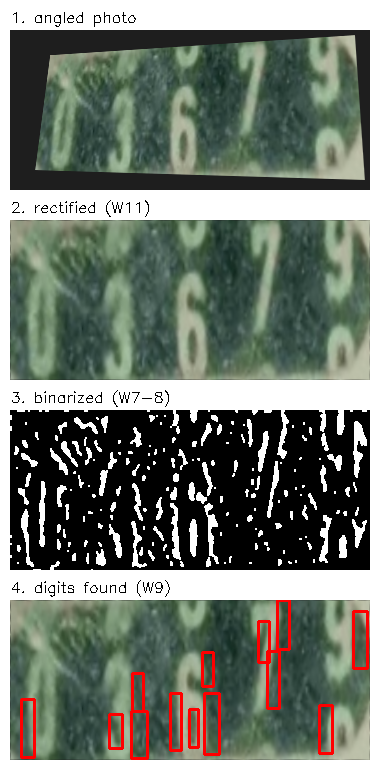
\includegraphics[height=0.82\textheight]{../assets/docscan_pipeline.png}
    \end{center}\end{column}
    \begin{column}{0.66\textwidth}
      \begin{itemize}
        \item \textbf{1. Photo} — a meter snapped at an angle (raw input).
        \item \textbf{2. Rectify} (W11) — homography warps it flat.
        \item \textbf{3. Binarize} (W2/7/8) — threshold + morphology clean it.
        \item \textbf{4. Segment} (W9) — contours find each digit box.
        \item \textbf{5. Read} (W13) — a CNN classifies each digit $\rightarrow$ ``03679''.
      \end{itemize}
    \end{column}
  \end{columns}
\end{frame}

\begin{frame}{Every week was a stage}
  \begin{center}
  \begin{tabular}{@{}ll@{}}
    \toprule
    \textbf{Weeks} & \textbf{DocScan role} \\
    \midrule
    1--4 Pixels, histograms, filtering, denoise & clean the raw photo \\
    5--6 Edges, Fourier & find structure, remove periodic noise \\
    7--9 Morphology, segmentation, contours & isolate the digits \\
    10--11 Features, homography & rectify to a flat scan \\
    12--16 ML, CNNs, transfer learning & read the digits \\
    \bottomrule
  \end{tabular}
  \end{center}
  \keyidea{DocScan isn't a separate project — it's the spine that every week added a vertebra to.}
\end{frame}

\begin{frame}[fragile]{The pipeline as one function (code)}
\begin{lstlisting}
def docscan(photo):
    warped = rectify(photo)                 # W11: homography + RANSAC
    if warped.inliers < 12:                 # confidence gate
        return Reject("blurry / bad angle - retake")
    binary = clean(warped.image)            # W2/7/8: threshold + morphology
    boxes  = segment_digits(binary)         # W9: contours -> ordered boxes
    if len(boxes) != EXPECTED_DIGITS:       # sanity check
        return Reject("wrong digit count")
    digits = [read_digit(b) for b in boxes] # W13 / transfer features
    return "".join(d.label for d in digits)
\end{lstlisting}
  \begin{itemize}
    \item Each helper is a week of the course; the glue is engineering.
  \end{itemize}
\end{frame}

\begin{frame}{Ordering the digit boxes}
  \begin{columns}[T]
    \begin{column}{0.52\textwidth}
      \begin{itemize}
        \item Contours come back in \emph{arbitrary} order — you must sort left-to-right.
        \item After rectification, sort boxes by their center $x$.
        \item Guard against split/merged blobs by checking width and spacing.
      \end{itemize}
    \end{column}
    \begin{column}{0.48\textwidth}
      \begin{center}
      \pixelgrid{{0,3,6,7,9}}
      \end{center}
      {\scriptsize sorted by center-$x$ $\rightarrow$ reading order ``03679''}
      \begin{badbox}
        Skip the sort and ``03679'' becomes ``73096''. Ordering is not optional.
      \end{badbox}
    \end{column}
  \end{columns}
\end{frame}

% ==================================================================
\section{Engineering for the real world}
% ==================================================================

\begin{frame}{Engineering a robust pipeline}
  \begin{itemize}
    \item \term{Confidence gates}: if RANSAC inliers are too few, ask for a new photo (don't guess).
    \item \term{Sanity checks}: a meter reading has a fixed number of digits — reject wrong counts.
    \item \term{Fallbacks}: if the feature path fails, try the contour path (and vice-versa).
    \item \term{Logging}: record per-stage quality (RMSE, digit confidences) to debug failures.
  \end{itemize}
  \begin{badbox}
    A demo works on one clean image; a product survives blur, glare, tilt, and dirt. Design for failure.
  \end{badbox}
\end{frame}

\begin{frame}{Confidence gating, quantified}
  \begin{columns}[T]
    \begin{column}{0.54\textwidth}
      \begin{mathbox}[Per-read confidence]
        A softmax digit read gives $p_1 \ge p_2 \ge \dots$. Gate on the \emph{margin}:
        \[ m = p_1 - p_2 \]
        Accept only if $m > \tau$ (e.g.\ $\tau=0.3$); else flag for review.
      \end{mathbox}
    \end{column}
    \begin{column}{0.46\textwidth}
      \begin{itemize}
        \item High $p_1$ but small margin = the net is torn between two digits.
        \item One low-margin digit taints the whole reading — gate per digit.
        \item Raising $\tau$ trades \emph{coverage} for \emph{precision}.
      \end{itemize}
    \end{column}
  \end{columns}
\end{frame}

\begin{frame}{The precision / coverage trade-off}
  \begin{columns}[T]
    \begin{column}{0.5\textwidth}
      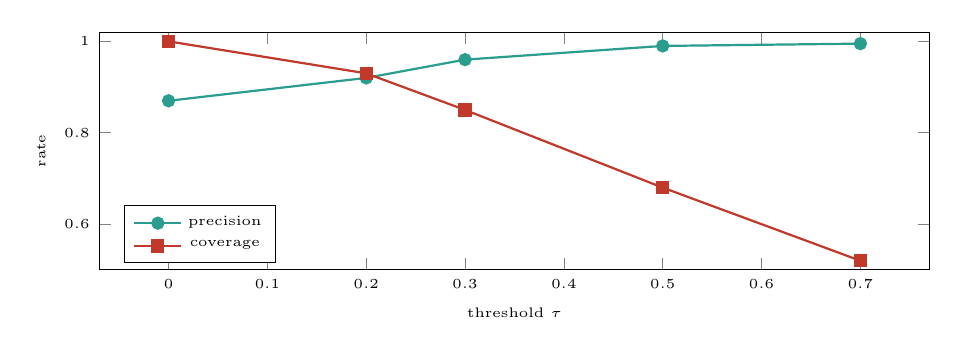
\begin{tikzpicture}[font=\tiny]
        \begin{axis}[width=\linewidth,height=4.6cm,
            xlabel={threshold $\tau$},ylabel={rate},
            ymin=0.5,ymax=1.02,legend pos=south west,legend style={font=\tiny}]
          \addplot[courseGood,thick,mark=*] coordinates
            {(0.0,0.87)(0.2,0.92)(0.3,0.96)(0.5,0.99)(0.7,0.995)};
          \addlegendentry{precision}
          \addplot[courseBad,thick,mark=square*] coordinates
            {(0.0,1.0)(0.2,0.93)(0.3,0.85)(0.5,0.68)(0.7,0.52)};
          \addlegendentry{coverage}
        \end{axis}
      \end{tikzpicture}
    \end{column}
    \begin{column}{0.5\textwidth}
      \begin{itemize}
        \item Raise $\tau$: fewer readings, but the ones you keep are more reliable.
        \item Billing wants \emph{precision}; a triage tool may want \emph{coverage}.
        \item Pick $\tau$ from the cost of a wrong bill vs.\ a re-scan.
      \end{itemize}
      \begin{goodbox}
        State your operating point: ``at $\tau=0.3$, 96\% precision over 85\% of photos.''
      \end{goodbox}
    \end{column}
  \end{columns}
\end{frame}

\begin{frame}{Fallbacks and graceful failure}
  \begin{columns}[T]
    \begin{column}{0.52\textwidth}
      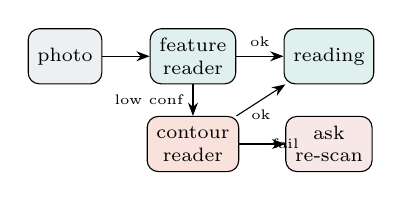
\begin{tikzpicture}[font=\scriptsize,>=Stealth,node distance=4mm and 6mm,
        b/.style={draw,rounded corners,align=center,minimum height=7mm,fill=coursePrimary!8}]
        \node[b](in){photo};
        \node[b,right=of in,fill=courseGood!15](main){feature\\reader};
        \node[b,below=of main,fill=courseAccent!20](fb){contour\\reader};
        \node[b,right=of main,fill=courseGood!15](ok){reading};
        \node[b,below=of ok,fill=courseBad!12](rej){ask\\re-scan};
        \draw[->](in)--(main);
        \draw[->](main)-- node[above,font=\tiny]{ok}(ok);
        \draw[->](main)-- node[left,font=\tiny]{low conf}(fb);
        \draw[->](fb)-- node[below,font=\tiny]{ok}(ok);
        \draw[->](fb)-- node[right,font=\tiny]{fail}(rej);
      \end{tikzpicture}
    \end{column}
    \begin{column}{0.48\textwidth}
      \begin{itemize}
        \item Two independent readers rarely fail on the \emph{same} image.
        \item If both disagree or gate out, \emph{refuse} — don't emit a guess.
        \item A refusal is cheap; a wrong bill is expensive and erodes trust.
      \end{itemize}
    \end{column}
  \end{columns}
\end{frame}

% ==================================================================
\section{In-class exercise}
% ==================================================================

\begin{frame}{\faPen~In-class exercise (10 min)}
  \begin{infobox}[Design the system]
  \end{infobox}
  \begin{enumerate}
    \item In DocScan, the rectify step returns very few RANSAC inliers. What should the system do?
    \item Your digit reader outputs $p_1=0.95$, $p_2=0.90$ for one digit. Accept it? Why?
    \item Segmentation returns 4 boxes but meters have 5 digits. What now?
    \item You want to guarantee correct bills. Do you raise or lower the confidence threshold?
  \end{enumerate}
\end{frame}

\begin{frame}{\faPen~Debrief}
  \begin{itemize}
    \item (1) \term{Gate it}: treat rectification as unreliable and prompt for a new photo rather than reading a bad scan.
    \item (2) \term{No} — the margin $m=0.05$ is tiny; the net is unsure between two digits. Flag for review.
    \item (3) \term{Reject / re-segment}: the digit-count sanity check failed; don't emit a 4-digit reading.
    \item (4) \term{Raise} $\tau$ — higher precision, fewer but more trustworthy readings.
  \end{itemize}
  \keyidea{Honest \emph{failure handling} beats a fancier model — a system that knows when it doesn't know is worth shipping.}
\end{frame}

\begin{frame}{A latency budget}
  \begin{columns}[T]
    \begin{column}{0.5\textwidth}
      \begin{tabular}{@{}lc@{}}
        \toprule
        \textbf{Stage} & \textbf{Time (ms)} \\
        \midrule
        rectify (homography) & 8 \\
        clean + morphology & 5 \\
        segment contours & 4 \\
        feature extraction (backbone) & 45 \\
        SVM classify $\times$5 digits & 3 \\
        \midrule
        \textbf{total} & \textbf{$\approx$65} \\
        \bottomrule
      \end{tabular}
    \end{column}
    \begin{column}{0.5\textwidth}
      \begin{itemize}
        \item The \emph{backbone} dominates — that's where transfer's cost lives.
        \item On-device, swap to a smaller backbone or quantize to hit a budget.
        \item Measure before optimizing; the contour path is nearly free.
      \end{itemize}
      \begin{goodbox}
        Profile per stage. You can't shrink what you never timed.
      \end{goodbox}
    \end{column}
  \end{columns}
\end{frame}

\begin{frame}{Common capstone pitfalls}
  \begin{itemize}
    \item \term{Preprocessing mismatch}: your resize/normalize differs from the backbone's — accuracy silently drops.
    \item \term{Data leakage}: same meter appears in train and test, or the scaler saw test data.
    \item \term{Unsorted digits}: correct classes, wrong order — a subtle, common bug.
    \item \term{No test number}: a demo on one image is not an evaluation.
  \end{itemize}
  \begin{badbox}
    Each of these can turn a real 0.87 into a fake 0.99 or a mysterious 0.40. Check them first.
  \end{badbox}
\end{frame}

% ==================================================================
\section{Course wrap-up}
% ==================================================================

\begin{frame}{The arc of the course}
  \begin{itemize}
    \item We started with a single pixel and ended with a pretrained neural network.
    \item Classical IP (weeks 1--11): precise, interpretable, no training — still essential for geometry \& cleanup.
    \item Learning (weeks 12--16): powerful for recognition, especially via transfer learning.
    \item \alert{A real system uses both}: classical to prepare, learned to recognize.
  \end{itemize}
\end{frame}

\begin{frame}{Choosing the right tool}
  \begin{center}
  \begin{tabular}{@{}ll@{}}
    \toprule
    \textbf{If you need to\ldots} & \textbf{Reach for\ldots} \\
    \midrule
    align/rectify/measure geometry & classical (homography, contours) \\
    clean noise, threshold, morphology & classical filters \\
    recognize with small data & transfer learning \\
    recognize with big data & train/fine-tune a CNN \\
    \bottomrule
  \end{tabular}
  \end{center}
  \keyidea{The mark of an engineer: picking the simplest tool that solves the problem reliably.}
\end{frame}

\begin{frame}{Honesty, ethics, and limits}
  \begin{itemize}
    \item Report the \emph{test} number, the failure cases, and the data you trained on — not just the best demo.
    \item A misread meter digit is a wrong bill; know your error rate and gate low-confidence reads.
    \item Beware dataset bias: if all training meters are clean and bright, expect failure on dirty ones.
  \end{itemize}
  \begin{badbox}
    ``97\% accurate'' means nothing without: on what data, which metric, and how it fails.
  \end{badbox}
\end{frame}

\begin{frame}{A quick self-check on the whole course}
  \begin{itemize}
    \item Can you clean a noisy image (denoise, threshold, morphology)? (W1--8)
    \item Can you find and measure shapes/contours? (W9)
    \item Can you rectify a tilted photo with a homography? (W10--11)
    \item Can you build a features$\rightarrow$classifier and a CNN, and use transfer learning? (W12--16)
  \end{itemize}
  \keyidea{If yes to all four, you can build the majority of practical vision systems end to end.}
\end{frame}

\begin{frame}{Where to go next}
  \begin{itemize}
    \item \term{Detection} (YOLO, Faster-RCNN): find \emph{and} locate objects — the next step past classification.
    \item \term{Segmentation} (U-Net, SAM): label every pixel — for your power-line/mask datasets.
    \item \term{OCR} systems (Tesseract, TrOCR): full text reading pipelines built on these ideas.
    \item \term{Deployment}: on-device (TFLite, ONNX), latency, and robustness in the field.
  \end{itemize}
\end{frame}

% ==================================================================
\section{The deliverable}
% ==================================================================

\begin{frame}{The capstone deliverable}
  \begin{alertblock}{Final project (see \code{capstone/})}
    \begin{enumerate}
      \item Assemble the full DocScan pipeline on real \code{E:/data} images.
      \item Rectify (W11) $\rightarrow$ clean/segment (W7--9) $\rightarrow$ read digits (W13 or transfer).
      \item Add at least two robustness features (confidence gate, digit-count check, fallback).
      \item Report end-to-end accuracy and where it fails; propose one concrete improvement.
    \end{enumerate}
  \end{alertblock}
\end{frame}

\begin{frame}{How your capstone is judged}
  \begin{columns}[T]
    \begin{column}{0.5\textwidth}
      \begin{tabular}{@{}lc@{}}
        \toprule
        \textbf{Criterion} & \textbf{Weight} \\
        \midrule
        Working end-to-end pipeline & 40\% \\
        Robustness features (2+) & 20\% \\
        Honest evaluation \& failure analysis & 25\% \\
        Clarity of report \& code & 15\% \\
        \bottomrule
      \end{tabular}
    \end{column}
    \begin{column}{0.5\textwidth}
      \begin{goodbox}
        A modest pipeline with an honest error analysis beats a flashy demo with no test number.
      \end{goodbox}
      \begin{badbox}
        No confidence gate + one cherry-picked image = an automatic re-do.
      \end{badbox}
    \end{column}
  \end{columns}
\end{frame}

\begin{frame}{A reproducibility checklist}
  \begin{columns}[T]
    \begin{column}{0.5\textwidth}
      \begin{goodbox}[Before you submit]
        \begin{itemize}
          \item Fixed random seed; train/test split saved.
          \item Backbone + preprocessing pinned to versions.
          \item One command reruns the whole pipeline.
        \end{itemize}
      \end{goodbox}
    \end{column}
    \begin{column}{0.5\textwidth}
      \begin{itemize}
        \item A result nobody can rerun is a claim, not evidence.
        \item Log the test number, the threshold $\tau$, and the failure cases together.
        \item Future-you (and your grader) should get the same number twice.
      \end{itemize}
    \end{column}
  \end{columns}
  \keyidea{If it doesn't reproduce, it didn't happen. Ship the recipe, not just the result.}
\end{frame}

\begin{frame}[standout]
  From one pixel to a working scanner.\\[4pt]
  \normalsize Classical vision to prepare, deep learning to recognize — and the judgment to know which, when.
\end{frame}

\end{document}
